\section{D. Shuffles}

\begin{frame} % No title at first slide
    \sectiontitle{D}{Shuffles}
    \sectionmeta{
        \texttt{math, adhoc}\\
        출제진 의도 -- \textbf{\color{acgold}Gold4}
    }
    \begin{itemize}
        \item 제출 ??번, 정답 ??명 (정답률 ??.??\%)
        \item 처음 푼 사람: \textbf{??}, ??분
    \end{itemize}
\end{frame}

\begin{frame}{\textbf{D}. Shuffles}
    \begin{itemize}
        \item 한 가지 관찰을 해봅시다. 예제 입력2 배열의 $x$축을 인덱스, $y$축을 값으로 한 그래프입니다.
        \begin{center}
            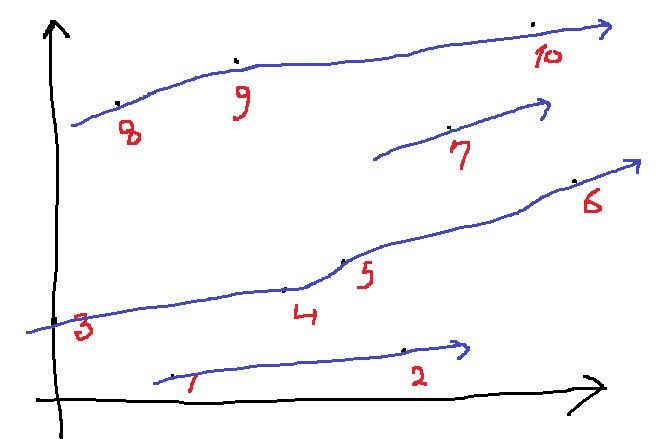
\includegraphics[width=0.6\linewidth]{../images/shuffles.png}
        \end{center}
    \end{itemize}
\end{frame}

\begin{frame}{\textbf{D}. Shuffles}
    \begin{itemize}
        \item 각 shuffle마다 파란색 화살표의 개수를 최대 2배로 만들 수 있습니다.
        \item 그럼 이 화살표의 개수를 어떻게 \complexity{N}만에 구할 수 있을까요?
    \end{itemize}
\end{frame}

\begin{frame}{\textbf{D}. Shuffles}
    \begin{itemize}
        \item 각 숫자를 인덱스로, 위치를 값으로 하는 $pos$ 배열을 만들어봅시다.
        \item $arr = 1,2,7,3,8,9,4,5,10,6, pos = 0,1,3,6,7,9,2,4,5,8$ 처럼 만들 수 있습니다.
        \item 이 때, $pos[i] > pos[i+1]$의 개수($cnt$)를 구하면, $cnt+1$은 파란색 화살표의 개수입니다.
        \item $cnt+1$ 이상인 가장 작은 $2^x$의 $x$가 답이 됩니다.
    \end{itemize}
\end{frame}